% TestingApparatus.tex
\subsection{Software Model} %or RED or DAQ etc
                        % check if \section and \subsubsection{}
                        % or \subsubsection and \subsubssection
                        % Methodology is \section so rest should be sub and subsub
This section provides an overview of the xyz.


\subsubsection{Functional Requirements}
% Contains a detailed list of what the system must do from the user's perspective. This includes user stories, use cases, and feature descriptions that clearly define system behaviors, inputs, outputs, and how users will interact with the system.

\subsubsection{Design Approach}
% Outlines the overall strategy for designing the system, including architectural patterns, design principles, and key technology choices. This explains the rationale behind major design decisions and how they align with requirements.

\subsubsection{Technical Specifications}
% Provides the detailed technical blueprint for implementation. Includes system architecture diagrams, data models, API definitions, algorithms, and specific technologies to be used. Translates the "what" into the "how" with precise technical parameters.

\subsubsection{Implementation Plan}
% Describes how the development will be executed, including task breakdown, timeline, resource allocation, and development methodology (Agile, Waterfall, etc.). Outlines milestones, dependencies, and critical path activities.


\subsubsection{Testing Strategy}
% Details the approach to validate that the system meets requirements. Includes test types (unit, integration, system, user acceptance), test environments, test data, automation approach, and quality metrics to ensure comprehensive coverage.


\subsubsection{Deployment Process}
% Specifies how the solution will be moved from development to production. Includes deployment steps, required environments, rollout strategy, rollback procedures, and post-deployment verification.

\subsubsection{Evaluation }
% Describes how system performance and user satisfaction will be measured. Includes success metrics, monitoring approach, feedback collection methods, and processes for incorporating learnings into future iterations.



%
% templates for figures, code, 
%

% %%% display code nicely
% \begin{lstlisting}[style=cstyle, caption=System Architecture Code Example, label=lst:SystemArchitecture7]
% # Your code here
% \end{lstlisting}

% \begin{figure}[htbp] %h-ere t-op b-ottom p-page (separte) -good to allow all htbp to give the compiler more options
%     \centering
%     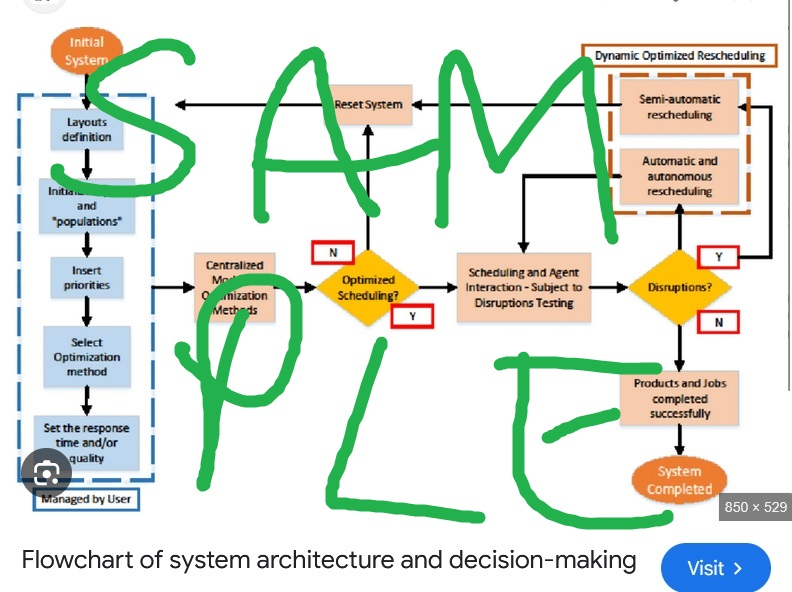
\includegraphics[width=0.6\textwidth]{figures/methodology/system_architecture.jpg}
%     \caption{System Architecture Diagram}
%     \label{fig:system-architecture2}
% \end{figure}

% % Include a flowchart in LATEX format
% \begin{figure}[H]
%     \centering
%     \scalebox{0.8}{ % Scale to 80% of original size
%         % try generating flowcharts as svg in Claude 
% and edit with inkscape instead of this.
% but claude did generate this one so might 
% be useful too but you can't easily make
% small repairs in inkscape


% CNN Transfer Learning Flowchart - Compact Multi-Column Layout
% \begin{figure}[htbp]

\centering
\resizebox{\textwidth}{!}{ % Scale to fit width while maintaining aspect ratio
\begin{tikzpicture}[node distance=0.8cm and 1.5cm, auto]
    % Define a smaller block style
    \tikzset{
      block/.style = {rectangle, draw, fill=blue!20, 
                      text width=7em, text centered, rounded corners, minimum height=1.8em, font=\small},
    }
    
    % Brazilian model training - Column 1
    \node [block] (brazildata) {Download Brazilian coins dataset};
    \node [block, below=of brazildata] (extract) {Extract dataset};
    \node [block, below=of extract] (setup) {Setup directories};
    \node [block, below=of setup] (define) {Define train/val dirs};
    \node [block, below=of define] (create) {Create CNN architecture};
    \node [block, below=of create] (compile) {Compile the CNN};
    \node [block, below=of compile] (train) {Train model};
    \node [block, below=of train] (trained) {Model trained (5 classes)};
    
    % Transfer learning - Column 2 (Middle)
    \node [block, right=2.5cm of brazildata] (freeze) {Freeze all layers};
    \node [block, below=of freeze] (replace) {Replace final layers};
    \node [block, below=of replace] (add) {Add regularization and dropout};
    \node [block, below=of add] (output) {New output layer (8 classes)};
    \node [block, below=of output] (finaltrain) {Train and fine-tune};
    \node [block, below=of finaltrain] (inference) {Perform inference on new coins};
    
    % UK data preparation - Column 3 (Right)
    \node [block, right=2.5cm of freeze] (ukdata) {Download UK coins dataset};
    \node [block, below=of ukdata] (ukextract) {Extract UK dataset};
    \node [block, below=of ukextract] (uksetup) {Setup UK directories};
    \node [block, below=of uksetup] (ukgen) {Create data generators (80/20 split)};
    
    % Connect all nodes with arrows
    \path [line] (brazildata) -- (extract);
    \path [line] (extract) -- (setup);
    \path [line] (setup) -- (define);
    \path [line] (define) -- (create);
    \path [line] (create) -- (compile);
    \path [line] (compile) -- (train);
    \path [line] (train) -- (trained);
    
    \path [line] (ukdata) -- (ukextract);
    \path [line] (ukextract) -- (uksetup);
    \path [line] (uksetup) -- (ukgen);
    
    % Connect the columns
    \path [line] (trained) -- node[midway, above] {Transfer} (freeze);
    \path [line] (ukgen) |- (finaltrain);
    
    % Connect middle column
    \path [line] (freeze) -- (replace);
    \path [line] (replace) -- (add);
    \path [line] (add) -- (output);
    \path [line] (output) -- (finaltrain);
    \path [line] (finaltrain) -- (inference);
    
    % Group boxes to show different stages with smaller padding
    \begin{pgfonlayer}{background}
        \node[group={[yshift=0.3cm]above:Brazilian Model Training}, fit={(brazildata) (extract) (setup) (define) (create) (compile) (train) (trained)}, inner sep=0.2cm] {};
        \node[group={[yshift=0.3cm]above:UK Data Preparation}, fit={(ukdata) (ukextract) (uksetup) (ukgen)}, inner sep=0.2cm] {};
        \node[group={[yshift=0.3cm]above:Transfer Learning}, fit={(freeze) (replace) (add) (output) (finaltrain) (inference)}, inner sep=0.2cm] {};
    \end{pgfonlayer}
\end{tikzpicture}
}
% \caption{CNN Transfer Learning Flowchart: Brazilian to UK Coins}
% \label{fig:cnn-flowchart}
% \end{figure}
%     }
%     \caption{System Design Overview Flowchart}
%     \label{fig:decriptiveLabel11} % descriptive to call in text with \ref{fig:decriptiveLabel}
% \end{figure}